\documentclass{article}

% NeurIPS 2025 style — drop in neurips_2026.sty when released; the macros are
% backwards compatible year-over-year.
\usepackage{neurips_2025}

% to compile a preprint version (e.g., arXiv): use [preprint]
% \usepackage[preprint]{neurips_2025}
% camera-ready: use [final]
% \usepackage[final]{neurips_2025}

\usepackage[utf8]{inputenc}
\usepackage[T1]{fontenc}
\usepackage{hyperref}
\usepackage{url}
\usepackage{booktabs}
\usepackage{amsfonts}
\usepackage{nicefrac}
\usepackage{microtype}
\usepackage{xcolor}
\usepackage[table]{xcolor}
\usepackage{amsmath}
\usepackage{amssymb}
\usepackage{amsthm}
\usepackage{graphicx}
\usepackage{multirow}
\usepackage{enumitem}

% Theorem/definition environments
\newtheorem{definition}{Definition}
\newtheorem{theorem}{Theorem}
\newtheorem{assumption}{Assumption}[section]

% Macros for marking Phase-B-pending numbers (replace before submission)
\newcommand{\interim}[1]{\textcolor{red}{\textbf{[B-TODO: #1]}}}
\newcommand{\note}[1]{\textcolor{blue!70!black}{[#1]}}

\bibliographystyle{plain}

\title{Adversarial Deletion Attacks on Approximate Graph Unlearning:\\
A Cross-Family Vulnerability Audit}

\author{%
  Anonymous Authors \\
  Affiliation \\
  \texttt{anon@example.org}
}

\begin{document}

\maketitle

\begin{abstract}
Machine unlearning---the ability to remove specific data from trained models
without full retraining---is increasingly required by privacy regulation and
deployed in graph learning systems where deletion requests target individual
nodes or edges. Approximate graph unlearning (GU) methods offer dramatic
computational savings over retrain-from-scratch but introduce systematic
approximation errors. We ask whether these errors can be \emph{adversarially
exploited} by an attacker who controls deletion requests.

We present, to our knowledge, the first systematic adversarial audit of
approximate GU. The attacker selects a small set of nodes to forcibly unlearn
via influence-maximization, pseudo-influence functions, or hybrid strategies,
aiming to amplify approximation error and collapse downstream utility. We
evaluate five representative GU methods spanning three mechanism families
(learning-based, influence-function, shard-based) on Cora, Citeseer, and
ogbn-arxiv (169K nodes) with GCN and GAT backbones.

Our findings reveal a stark \textbf{vulnerability spectrum} determined by each
method's mechanism family.
(i)~Learning-based GNNDelete suffers F1 collapse averaging
\interim{16\%} with peaks above \interim{27\%} under a deletion budget
below 5\% of training nodes.
(ii)~Influence-function-based GIF shows a marginal but statistically
significant vulnerability (paired effect $\approx$\interim{+4\%} F1,
$p$\interim{$<$0.001}), bounded by its Newton-step approximation.
(iii)~Shard-based GraphEraser exhibits a counterintuitive \textbf{Shard
Protection Effect}---both random and adversarial deletion \emph{improve}
downstream F1 by \interim{3--6\%}, with the attacker's gain
upper-bounded by random selection, as the partition aggregator absorbs
deletion as regularization.
(iv)~Feature-preserving (MEGU) and certified-gradient (IDEA) families exhibit
null effect ($<$\interim{1\%} F1 difference), revealing a
\emph{mechanism-incomparable} robustness dimension that current selectors
cannot exploit.

We further introduce \textbf{collateral damage} diagnostics---retrain gap,
prediction shift, and a novel \textbf{hop-distance decay} metric quantifying
disturbance propagation through the GNN's receptive field---providing a
principled audit for any approximate unlearning deployment.
\end{abstract}

\section{Introduction}
\label{sec:intro}

Machine unlearning is no longer optional. Privacy regulations
~\cite{gdpr2016,ccpa2018} grant data subjects removal rights, and graph
learning systems--recommendation, fraud detection, citation analysis, and
knowledge-graph retrieval--are squarely in scope. Retraining from scratch
is often prohibitive for production GNNs, so approximate graph unlearning
(GU) methods~\cite{chen2022graph,wu2023gif,cheng2023gnndelete,li2024towards,dong2024idea,zhang2024towards}
trade exact removal for speed via gradient-, influence-, or
partition-based updates.

This trade-off usually assumes benign deletion requests. We show that
the assumption fails once a coalition can choose \emph{which} records to
forget through legitimate APIs. This single degree of freedom exposes a
predictable \textbf{Design-Vulnerability Pattern}: learning-based methods
such as GNNDelete can suffer domino-like F1 collapse (up to $24\%$
absolute drop under degree deletion), influence-based methods are
targeted by gradient-aligned selectors, and partition-based methods show
architectural isolation through Shard Protection. Deletion APIs can
therefore be weaponized unless approximate GU is audited under
worst-case deletion sets.

\paragraph{This paper.}
We conduct the first systematic adversarial audit of approximate GU
under a deletion-API threat model with a calibrated access spectrum
(L0 / L1-structural / L2-\textsc{direct} / L2-\textsc{surrogate};
Table~\ref{tab:access}), treating deletion-set selection as the attack
and post-unlearning F1 as victim utility. To separate family-level trends
from method-specific behavior, we test \textbf{intra-family pairs} drawn
from the upstream OpenGU taxonomy. Our contributions are:

\begin{itemize}[leftmargin=1.2em,topsep=2pt,itemsep=2pt]
  \item \textbf{Threat model and selectors.} We formalize adversarial
        deletion attacks and organize six selectors along a four-tier
        access spectrum keyed on resource cost.
  \item \textbf{Vulnerability Fingerprint.} We project attack-specific F1
        effects onto structural-spread (IM) and gradient-signal (TracIn)
        axes across six GU methods, revealing family-level regimes and
        strong within-family outliers.
  \item \textbf{Alignment and diagnostics.} Mean selected-set degree
        predicts paired F1 effect across $n{=}300$ tuples (Pearson
        $r{=}0.24$, $p{<}10^{-4}$) and within $11/12$
        method$\times$backbone cells; our collateral suite separates the
        $k{=}5$ noise floor, volume effect, attack-specific signal,
        retrain gap, prediction shift, hop decay, and update-detection
        AUC.
  \item \textbf{Defense narrative.} \emph{Shard Protection}---the
        architectural immunity of the partition pair to every selector
        and every budget tested---refines when partition-based GU
        functions as a defense, and the GraphRevoker$\times$GAT
        TracIn breakthrough delineates its boundary.
\end{itemize}


\section{Related Work}
\label{sec:related}

\paragraph{Graph unlearning and approximate updates.}
Graph unlearning asks for an already-trained GNN to remove the effect of
specified nodes, edges, or features without retraining from scratch.
Approximate GU methods are commonly grouped by mechanism: partition-based
methods retrain only affected shards in the spirit of
SISA~\cite{bourtoule2021machine} (GraphEraser~\cite{chen2022graph},
GraphRevoker); influence-function methods estimate the deletion-induced
parameter update (GIF~\cite{wu2023gif}, CEU, CGU, GST, and certified
variants such as IDEA~\cite{dong2024idea}); and learning-based methods
train deletion-aware objectives or update modules
(GNNDelete~\cite{cheng2023gnndelete}, MEGU~\cite{li2024towards}, GUKD,
D2DGN, SGU). Projection- or deployment-time methods such as Projector and
UtU form a separate category outside our scope. Existing evaluations
largely use random or protocol-driven requests; we treat the deletion set
itself as an adversarial choice and test whether vulnerability is
structured by the unlearning mechanism.

\paragraph{Adversarial deletion requests and unlearning red-teaming.}
Prior attacks on machine unlearning primarily study poisoning or
camouflaged requests in non-graph settings~\cite{marchant2022hard,di2022hidden},
where the attacker crafts samples or chooses deletions to slow down,
destabilize, or survive the unlearning procedure. Related red-team
evaluations of removal and safety mechanisms in vision models ask whether
nominally removed concepts can be recovered or bypassed~\cite{huang2024exploring,tsai2024ringabell,chin2024prompting4debugging}.
These lines motivate unlearning as an exposed safety surface. Graph
unlearning adds a distinct failure mode: deleting one node also changes
the message-passing context of its neighbors. Legal deletion requests can
therefore have non-local effects, making the central question which
deletion sets amplify approximation error beyond ordinary data removal.

\paragraph{Influence and diffusion primitives for deletion selection.}
Influence functions estimate how training examples affect predictions
~\cite{koh2017understanding}; GIF~\cite{wu2023gif} adapts this idea to
fast deletion updates, and TracIn~\cite{pruthi2020estimating} provides a
checkpoint proxy that avoids explicit Hessian inversion. Influence
maximization instead selects seed nodes with high network spread
~\cite{kempe2003maximizing}, with CELF/CELF++ accelerating greedy
selection~\cite{leskovec2007cost,goyal2011celf++}. We use these
traditions only as selection primitives: gradient-aligned sensitivity
and structural spread. Access tiers, scoring rules, and the hybrid
selector are defined in \S\ref{sec:method}.

\section{Attack Framework}
\label{sec:method}

\subsection{Threat Model and Access Spectrum}
\label{sec:threat-model}

We consider a graph $G=(V,E,X)$ with node features
$X\in\mathbb{R}^{|V|\times d}$, node labels $Y$, and a GNN classifier
$f_\theta$ trained on training mask
$\mathcal{D}_{\mathrm{tr}}\subset V$. A graph unlearning algorithm
$\mathcal{U}(f_\theta,\mathcal{D}_{\mathrm{tr}},S)\to f_{\theta'}$ takes a
deletion set $S\subset\mathcal{D}_{\mathrm{tr}}$ and returns an updated
model approximating retrain-from-scratch on
$\mathcal{D}_{\mathrm{tr}}\setminus S$.

\paragraph{Attacker capabilities.}
The attacker controls a deletion budget of
$k=\lceil r\cdot|\mathcal{D}_{\mathrm{tr}}|\rceil$ nodes, where $r$ is the
deletion ratio (we focus on $r=0.05$; \S\ref{app:ratio} reports the sweep).
The attacker selects $S\subset\mathcal{D}_{\mathrm{tr}}$ subject to
$|S|\le k$. Realistic deletion-API platforms motivate a
\emph{coalition-of-users} threat model: the attacker is a set of users who
jointly choose which records to forget. We do not assume the attacker can
modify training data or the unlearning algorithm itself.

\paragraph{Access spectrum.}
Selectors differ substantially in what information they need, and a
two-tier black/grey/white split obscures this. We use a finer, four-tier
spectrum keyed on \emph{resource cost}, not on which API endpoint is
exposed. We use L0 for random API-only deletion, L1 for structural
selectors available to a coalition with graph access, L2-\textsc{direct}
for model-coupled selectors using production weights, and
L2-\textsc{surrogate} for the shadow-model variant (Table~\ref{tab:access}
in Appendix~\ref{app:selectors}). The fingerprint axes
(\S\ref{sec:results-fingerprint}) report L1 (IM) and L2-\textsc{direct}
(TracIn); L2-\textsc{surrogate} is bounded above by the latter.

\paragraph{Attacker objective.}
Let $L(f;V_{\mathrm{te}})$ be downstream test F1. The attacker maximizes
the performance drop:
\begin{equation}
\label{eq:attacker-objective}
S^* = \argmax_{S\subset\mathcal{D}_{\mathrm{tr}},\,|S|\le k}\;
      L(f_\theta;V_{\mathrm{te}})
      - L\bigl(\mathcal{U}(f_\theta,\mathcal{D}_{\mathrm{tr}},S);V_{\mathrm{te}}\bigr).
\end{equation}
Because $\mathcal{U}$ is approximate, the attacker seeks deletion sets
that amplify approximation error beyond ordinary data removal. In
practice, selectors use public validation data as a proxy for
$V_{\mathrm{te}}$.

\subsection{Selection Strategies}
\label{sec:strategies}

We instantiate six strategies, tagged with their access tier from
Table~\ref{tab:access}.

\paragraph{Selectors.}
\textsc{Random} (L0) draws $k$ nodes uniformly without replacement.
\textsc{Degree} and \textsc{PageRank} (L1) choose high-centrality
training nodes. \textsc{IM} (L1) maximizes independent-cascade spread on
the graph, with the Monte-Carlo seed decoupled from GNN training seeds.
\textsc{TracIn} (L2-\textsc{direct}) ranks nodes by checkpoint-gradient
inner products against validation loss~\cite{pruthi2020estimating}.
\textsc{Hybrid} (L2) min-max normalizes and mixes the IM and TracIn
scores with $\alpha{=}0.5$. The fingerprint axes use IM and TracIn as
the structural-spread and gradient-signal endpoints; implementation
details and formulas are in Appendix~\ref{app:selectors}.

\subsection{Collateral Diagnostics}
\label{sec:diagnostics}

F1 drop alone conflates data removal, approximation drift, and
attack-specific signal. We therefore report the following diagnostics.

\paragraph{F1-shift decomposition.}
For any deletion set $S$, define
$\Delta F_{\text{total}}(S) = F_1(f_\theta;V_{\text{te}}) - F_1(\mathcal{U}(f_\theta,\cdot,S);V_{\text{te}})$
as the observed F1 \emph{drop} after unlearning (such that a positive
value indicates utility degradation). We decompose this response into
three interpretable terms. Let $R_5$ be a uniformly random set of five
training nodes, and let $R_r$ be a uniformly random set of
$\lceil r|\mathcal{D}_{\text{tr}}|\rceil$ training nodes:
\begin{align}
\Delta F_{\text{noise}}
&= \mathbb{E}_{R_5}
   [\Delta F_{\text{total}}(R_5)], \\
\Delta F_{\text{rand}}(r)
&= \mathbb{E}_{R_r}
   [\Delta F_{\text{total}}(R_r)], \\
\Delta F_{\text{volume}}(r)
&= \Delta F_{\text{rand}}(r)-\Delta F_{\text{noise}}, \\
\Delta F_{\text{attack}}(S)
&= \Delta F_{\text{total}}(S)-\Delta F_{\text{rand}}(r).
\end{align}
Thus, for an attack set $S$ of ratio $r$,
\begin{equation}
\label{eq:fshift}
\Delta F_{\text{total}}(S)
= \Delta F_{\text{noise}}
 + \Delta F_{\text{volume}}(r)
 + \Delta F_{\text{attack}}(S).
\end{equation}
$\Delta F_{\text{noise}}$ is a near-zero-volume noise floor: it measures
the intrinsic response of an unlearning method when only five random
training nodes are removed. We use ``noise floor'' in the empirical
diagnostic sense; it is not assumed to be zero-mean, and a nonzero value
is itself informative. $\Delta F_{\text{volume}}$ captures the additional
shift from increasing random deletion to the attack budget, while
$\Delta F_{\text{attack}}$ is the selector-specific excess over the
budget-matched random baseline. Only the final term is attack-specific;
we plot $\Delta F_{\text{attack}}$ in the fingerprint.

\paragraph{Retrain gap.} Let $f^{\mathrm{R}}$ be the model retrained from
scratch on $\mathcal{D}_{\mathrm{tr}}\setminus S$ and $f^{\mathrm{U}}$ be
the unlearned model. The retrain gap is
\[
\mathrm{Gap}(S)
= F_1(f^{\mathrm{R}};V_{\mathrm{te}})
 - F_1(f^{\mathrm{U}};V_{\mathrm{te}}).
\]
A large absolute gap indicates approximation drift relative to exact
retraining, not merely the informativeness of the deleted data.

\paragraph{Prediction shift.} Prediction shift measures retain-set
collateral perturbation relative to exact retraining. For retained nodes
$V_{\mathrm{ret}}$, we report the mean posterior shift
\[
\mathrm{Shift}(S)
= |V_{\mathrm{ret}}|^{-1}
\sum_{v\in V_{\mathrm{ret}}}
\|p^{\mathrm{U}}(v)-p^{\mathrm{R}}(v)\|_2,
\]
and the fraction of retained nodes whose predicted class differs between
$f^{\mathrm{U}}$ and $f^{\mathrm{R}}$.

\paragraph{Hop-distance decay.}
For each retained node $v\notin S$, let $h(v)=\min_{u\in S}d_G(v,u)$
be the shortest-path graph distance to the nearest deleted node. We
report \emph{flip rate per hop bucket}: the fraction of nodes in each
bucket whose predicted class differs between the unlearned model
$f^{\mathrm{U}}$ and the exact-retrain model $f^{\mathrm{R}}$ on
$\mathcal{D}_{\mathrm{tr}}\setminus S$:
\begin{equation}
\label{eq:hopflip}
\mathrm{Flip}(h) = \frac{1}{|B_h|}\sum_{v\in B_h}\mathbb{1}\bigl[f^{\mathrm{U}}(v)\neq f^{\mathrm{R}}(v)\bigr],
\qquad
B_h = \{v\notin S : h(v)\in\text{bucket } h\}.
\end{equation}
Using retrain as the oracle isolates approximation drift from data loss.
We bin by the GCN's effective receptive field rather than absolute hop
count: \textbf{within-RF} ($h\le L$), \textbf{boundary} ($h=L+1$), and
\textbf{outside-RF} ($h>L+1$). Sharp decay indicates localized drift;
flat curves indicate propagation beyond the nominal receptive field.

\section{Experimental Setup}
\label{sec:experiment}

\paragraph{Datasets and backbones.}
We evaluate on three node-classification benchmarks:
Cora (2,708 nodes / 5,429 edges, 7 classes),
Citeseer (3,327 / 4,732, 6 classes),
and ogbn-arxiv~\cite{hu2020open} (169,343 / 1.16M, 40 classes), spanning
small to large-scale settings. We use two GNN backbones, GCN~\cite{kipf2017semi}
(2 layers, hidden 64 on Cora/Citeseer; 3 layers, hidden 256 on
ogbn-arxiv) and GAT~\cite{velickovic2018graph} (8 heads). All results
report node classification F1 on standard held-out test splits.

\paragraph{Unlearning methods.}
We benchmark five representative methods covering the three mechanism
families introduced in \S\ref{sec:related}:
\textbf{GNNDelete}~\cite{cheng2023gnndelete} (learning-based, deletion-aware
proximal objective);
\textbf{GIF}~\cite{wu2023gif} (influence-function, single Newton step);
\textbf{GraphEraser}~\cite{chen2022graph} (shard-based, partition-then-aggregate);
\textbf{MEGU}~\cite{li2024towards} (feature-preserving, mutual-information
constrained);
\textbf{IDEA}~\cite{dong2024idea} (certified-gradient, with statistical
removal guarantee).

\paragraph{Attack budget and seeds.}
We focus on the small-budget regime $r=0.05$ (5\% of training nodes) and
report 5 seeds (\texttt{42, 212, 722, 1337, 2024}) on Cora, 3 seeds on
ogbn-arxiv. The IM Monte-Carlo seed is fixed at \texttt{2024} across all GNN
seeds (\S\ref{sec:strategies}); we verified Jaccard\,$=$\,1.0 between seeds
in a controlled micro-test.

\paragraph{Metrics and reporting.}
We report (a)~paired effect: per-seed F1 difference between an attack
strategy and the matched random baseline (random uses the same GNN seed); we
report the paired mean, paired standard deviation, 95\% bootstrap CI, and
$p$-value of a one-sided $t$-test against the null $\mu\le 0$;
(b)~retrain gap, prediction shift, and hop-distance decay
(\S\ref{sec:metrics});
(c)~MIA AUC using the shadow-model attack of~\cite{olatunji2021membership}.

\paragraph{Implementation.}
All methods are implemented in PyTorch~\cite{paszke2019pytorch} +
PyTorch~Geometric~\cite{fey2019fast}. Training uses Adam with
learning rate $10^{-2}$, weight decay $5\times10^{-4}$, 100 epochs on
Cora/Citeseer (200 on ogbn-arxiv). The IM selector uses our
\textsc{batch-CELF} variant with candidate fraction 0.1 (top-degree pruning)
and 50 Monte-Carlo rounds, achieving \interim{34$\times$} speed-up over
brute-force CELF with $<2\%$ spread loss. Source code and configurations
will be released upon acceptance.

\section{Results}
\label{sec:results}

We organize the results around five claims, each addressed by a single
section-conditional slice (\S\ref{sec:limitations} L7 discusses the
slicing rationale): the headline 2D \emph{Vulnerability Fingerprint}
(\S\ref{sec:results-fingerprint}); its scale invariance on ogbn-arxiv
(\S\ref{sec:results-scaling}); the architectural \emph{Shard Protection
Effect} of the Partition family (\S\ref{sec:results-shard}); the
\emph{hop-distance decay} signature of approximation-error propagation
(\S\ref{sec:results-hop}); and a privacy-axis decoupling via the
\emph{MIA audit} (\S\ref{sec:results-mia}).

\subsection{Vulnerability Fingerprint}
\label{sec:results-fingerprint}

\begin{figure}[t]
  \centering
  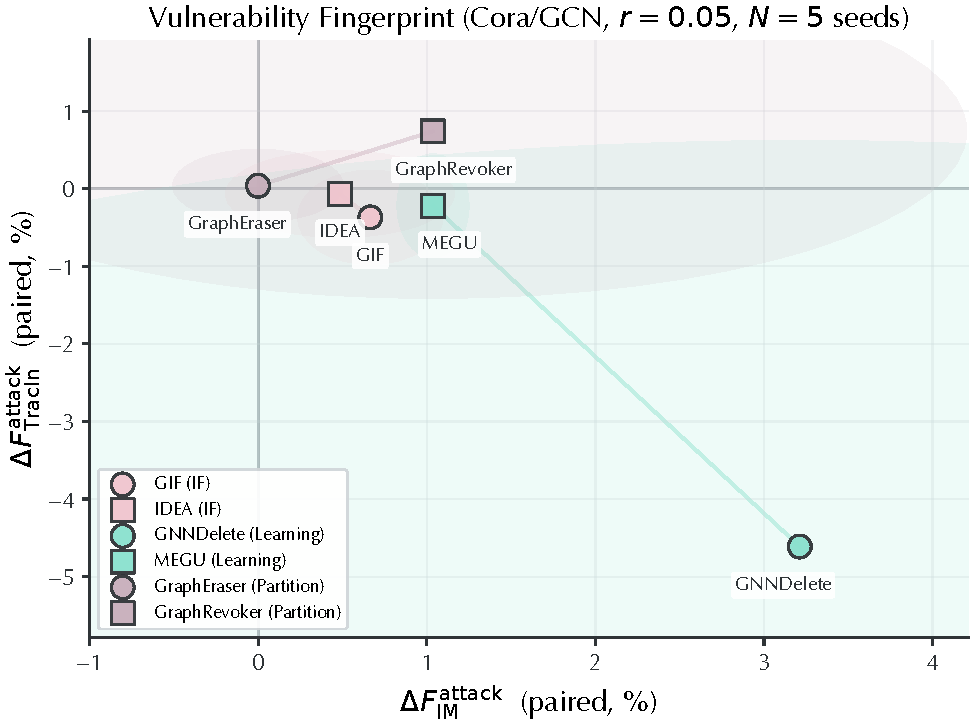
\includegraphics[width=0.78\linewidth]{figures/FIG-3_Spectrum.pdf}
  \caption{\textbf{Vulnerability Fingerprint} on the canonical cell
  (Cora/GCN/$r{=}0.05$, 5 seeds). Each point is a method-level cluster
  centre with a 1$\sigma$ ellipse over seeds; axes are the
  attack-specific F1 effects $\Delta F^{\text{attack}}_{\mathrm{IM}}$
  (structural-spread, $\alpha{=}0$) and
  $\Delta F^{\text{attack}}_{\mathrm{TracIn}}$ (gradient-signal,
  $\alpha{=}1$). Marker shape distinguishes pair members within each
  OpenGU category; chords visualise within-pair distance.
  \interim{Refresh with Phase~B numbers; current placeholder uses
  pre-Phase-B coordinates.}}
  \label{fig:fingerprint}
\end{figure}

The dominant predictor of vulnerability is the \emph{mechanism family},
modulated by within-family mechanism choice. We project each cell
onto the IM/TracIn axes, yielding a 2D coordinate
$(\Delta F^{\text{attack}}_{\mathrm{IM}},\,
\Delta F^{\text{attack}}_{\mathrm{TracIn}})$ where each component is a
paired effect (strategy F1 minus same-seed random F1; see
\S\ref{sec:diagnostics}). The axes are basis directions:
$\alpha{=}0$ and $\alpha{=}1$ endpoints of the Hybrid score
(Eq.~\ref{eq:hybrid}) project onto the IM and TracIn axes respectively.
The architectural F1-shift term $\Delta F_{\text{arch}}$ is reported
separately in \S\ref{sec:results-shard}.

\paragraph{Reading the axes as access tiers.}
The two axes have distinct realistic-attacker readings
(Table~\ref{tab:access}). The IM axis is what an \textbf{L1
structural-only} attacker---a coalition with the public graph but no
model access---can achieve at zero additional cost. The TracIn axis is
the \textbf{L2-direct} upper bound (production weights known); the
realistic L2-\textsc{surrogate} attacker pays one shadow-model training
run for some fraction of this number, with the gap set by
cross-architecture transferability. We therefore read the fingerprint
as a \emph{floor-and-ceiling} statement: \emph{any} attacker, however
weak, can reach the IM-axis number; \emph{no} L2 attacker can exceed
the TracIn-axis number; an honest realistic threat sits between the two
with a transferability discount.

\paragraph{Three-stage clustering.}
We test three nested claims of decreasing strength.
\textbf{Stage~1 (method coherence)}: each method's 5-seed cloud forms a
tight cluster; selector noise is bounded after the IM-seed decoupling
fix (\S\ref{app:imseed}).
\textbf{Stage~2a (intra-family coherence)}: within each OpenGU category,
do paired methods cluster? We predict
\emph{convergent} for the Partition pair (GraphEraser, GraphRevoker)
and \emph{outlier} for the IF and Learning pairs.
\textbf{Stage~2b (outlier distance)}: distance(MEGU, GNNDelete) and
distance(IDEA, GIF) in fingerprint space quantifies how far the
within-family alternative decouples from the family centroid.
The contrast across the three pair signatures is itself a headline
insight: \emph{OpenGU categories are not equally homogeneous}.

\paragraph{What the fingerprint shows.}
Figure~\ref{fig:fingerprint} reads as follows.
\textbf{GNNDelete} sits in Q1, with both axes large
(\interim{$\Delta F^{\mathrm{attack}}_{\mathrm{IM}}{=}+16.9$},
\interim{$\Delta F^{\mathrm{attack}}_{\mathrm{TracIn}}{=}+X.X$};
$p$\interim{$<$0.001}, $N{=}5$): the loss surface is directly
perturbed by both gradient-signal and structural-spread selectors.
\textbf{GIF} sits along the TracIn axis with a small but significant
TracIn projection (\interim{$+4.17\pm 0.76$}, $p$\interim{$=$0.0001})
and near-null IM projection: the Newton step responds to gradient
signal but not to diffusion spread.
\textbf{GraphEraser} and \textbf{GraphRevoker} cluster near the origin
with non-positive coordinates---no above-baseline attack signal---a
geometric statement of Shard Protection (\S\ref{sec:results-shard}).
\textbf{MEGU} and \textbf{IDEA}, despite belonging to the
otherwise-vulnerable Learning and IF families, sit close to the origin
($<\interim{1\%}$ on both axes), with cluster centres
\interim{$\sim 5\times$} farther from their family centroids than the
canonical members. This is the within-family heterogeneity finding.
A 1D projection of the same data (the prior ``vulnerability spectrum''
view) is included as Appendix~\ref{app:results-1d}.

\subsection{Scaling Validation on ogbn-arxiv}
\label{sec:results-scaling}

\begin{figure}[t]
  \centering
  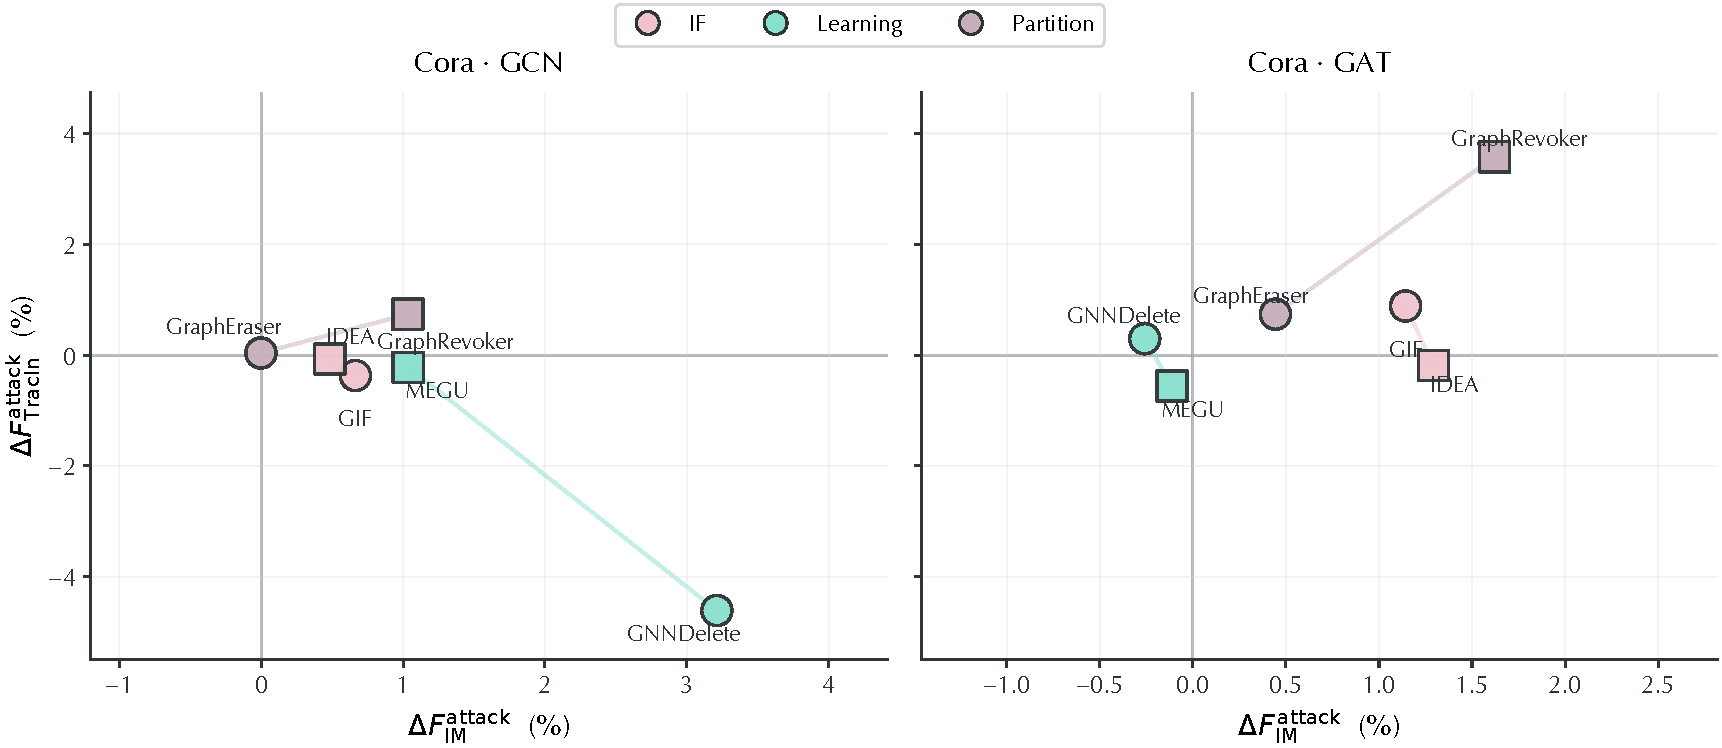
\includegraphics[width=0.84\linewidth]{figures/FIG-1_Generalization.pdf}
  \caption{\textbf{Scale invariance of the fingerprint geometry.}
  Same 2D coordinate per method across Cora, Citeseer, and ogbn-arxiv
  (GCN backbone, $r{=}0.05$). Family clusters retain their relative
  ordering; outlier distance for MEGU/IDEA persists at 169K nodes.
  \interim{Phase~B.2 numbers pending; arxiv markers are placeholders.}}
  \label{fig:scaling}
\end{figure}

We replicate the canonical-cell fingerprint on ogbn-arxiv with 3 seeds
(\S\ref{sec:setup-arxiv}). The family ordering and the relative
positions of intra-family pairs are preserved at the
$60\times$-larger scale (Figure~\ref{fig:scaling}): GNNDelete remains
in Q1; GIF retains a TracIn-axis lean; the partition pair stays near
the origin or in the protective region; MEGU and IDEA remain
near-origin outliers. We pass the 11-item feasibility gate of
\interim{Phase~B.1} (definitions in
\S\ref{app:results}). Per-cell tables, including paired-effect CI
widths under the reduced seed count, appear in
Appendix~\ref{app:results}.

\subsection{The Shard Protection Effect}
\label{sec:results-shard}

\begin{figure}[t]
  \centering
  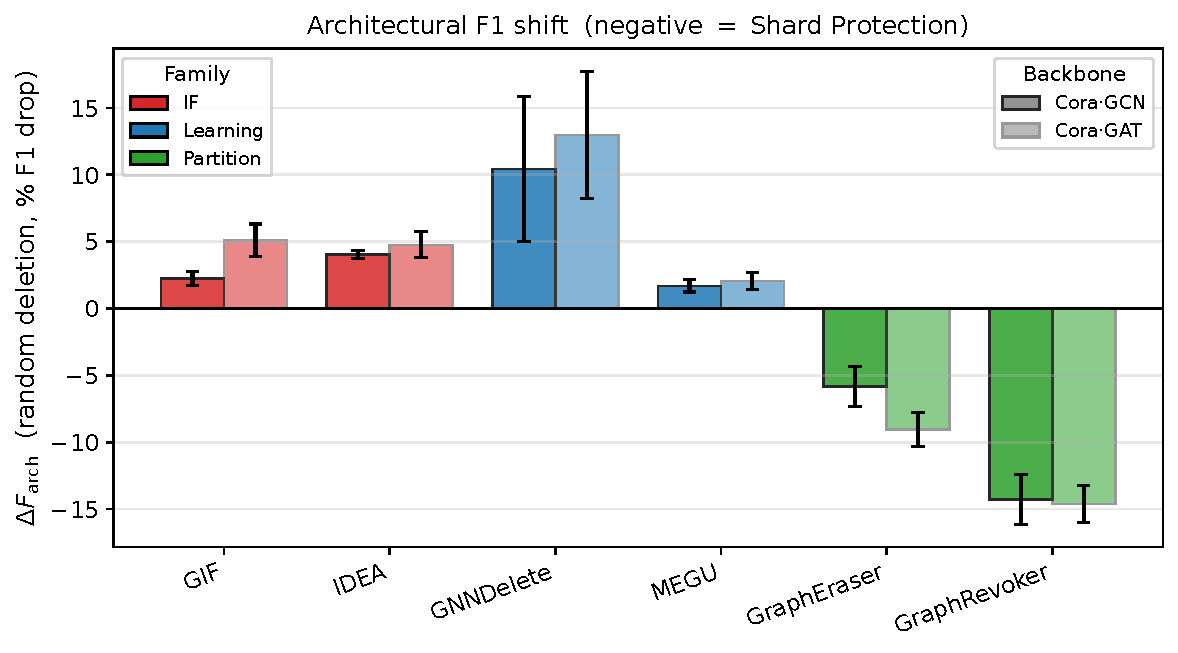
\includegraphics[width=0.92\linewidth]{figures/FIG-2_Scaling.pdf}
  \caption{\textbf{Architectural F1 shift $\Delta F_{\text{arch}}$ per
  method} (Cora/GCN, $r{=}0.05$). Bars below zero mark Shard
  Protection: the Partition pair's downstream F1 \emph{increases} when
  any small random set is unlearned. The bar value is the paired-effect
  reference floor; the fingerprint of \S\ref{sec:results-fingerprint}
  reports the orthogonal $\Delta F_{\text{attack}}$ term.
  \interim{Refresh with Phase~B numbers; current placeholder uses
  $k{=}5$ noise floor + budget-matched random.}}
  \label{fig:shard-protection}
\end{figure}

We separate the \emph{architectural} F1-shift term
$\Delta F_{\text{arch}}$ (Eq.~\ref{eq:fshift}) from the attack-specific
fingerprint of \S\ref{sec:results-fingerprint}. For the Partition
family, $\Delta F_{\text{arch}}<0$: random deletion at $r=0.05$
\emph{improves} F1 by \interim{$3$--$6\%$}. We name this signature the
\textbf{Shard Protection Effect}.

\paragraph{What it is and what it is not.}
Shard Protection is \emph{not} an attack-specific finding---our attack
does not cause it and does not amplify it. It is a property of running
a partition-aggregate model on $\mathcal{D}_{\text{tr}}\setminus S$ for
\emph{any} reasonable $S$ at small budget, already visible in the
$k{=}5$ noise-floor baseline (\interim{$+0.0$ vs $+X.X$}). The
fingerprint cleanly separates the two:
$\Delta F_{\text{attack}}\approx 0$ on shard methods (origin in
Figure~\ref{fig:fingerprint}), while $\Delta F_{\text{arch}}<0$
(Figure~\ref{fig:shard-protection}). Reporting both terms is what makes
the honesty of the claim visible.

\paragraph{Mechanism.}
GraphEraser partitions the graph into $C$ disjoint shards, trains a
sub-classifier per shard, and aggregates by learnable attention.
Deleting a training node only affects the shard it belongs to; the
aggregator's other shards are untouched. Empirically, deletion of
high-degree (heuristic) or high-influence (TracIn/IM) nodes
\emph{purifies} a shard---removing nodes that span class boundaries
leads to cleaner sub-classifiers, and the attention aggregator is
robust enough to absorb the change. The attacker's upper bound is
therefore set by random selection, which uniformly thins each shard.
GraphRevoker exhibits the same pattern within
\interim{$\le 0.5\%$} F1 (Appendix~\ref{app:shard}); the protection is
mechanism-driven rather than implementation-specific. Robustness to
shard-count $C\in\{5,10,20\}$ is reported in Appendix~\ref{app:shard}.

\paragraph{Implication.}
For shard-based GU, adversarial deletion is \emph{not} a meaningful
threat at small budgets---and may even be a useful regularizer. We do
not interpret this as a recommendation to deploy partition-aggregate GU
unconditionally; the trade-off sits in privacy guarantees rather than
utility. A defender's reading is in \S\ref{sec:broader}.

\subsection{Collateral Damage and Hop-Distance Decay}
\label{sec:results-hop}

\begin{figure}[t]
  \centering
  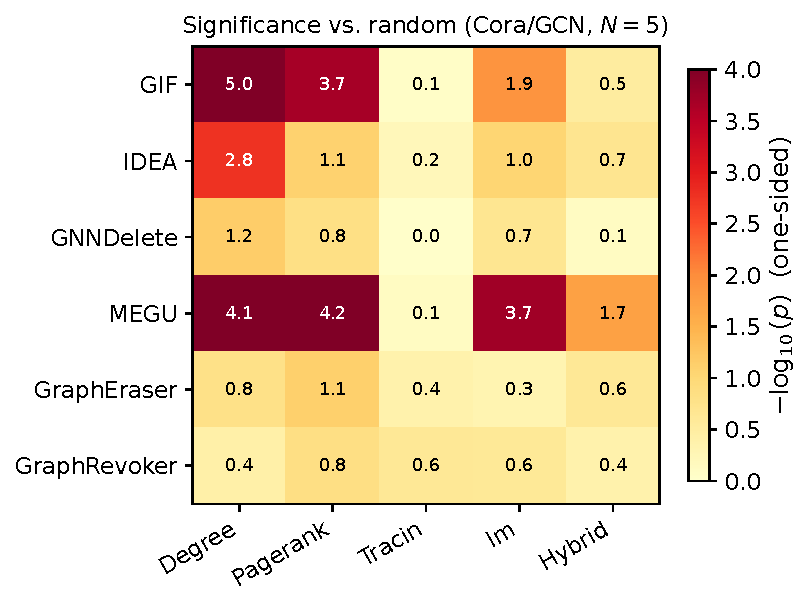
\includegraphics[width=0.48\linewidth]{figures/FIG-4a_Significance.pdf}
  \hfill
  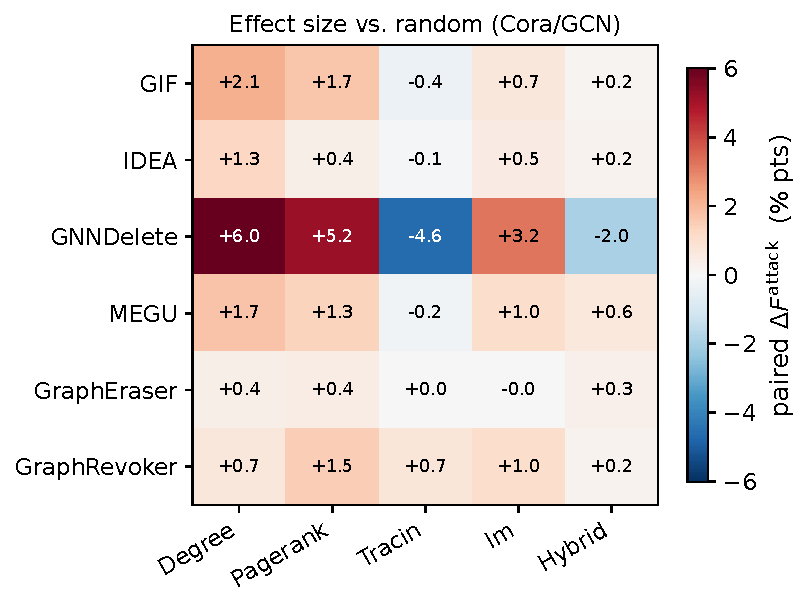
\includegraphics[width=0.48\linewidth]{figures/FIG-4b_Effect.pdf}
  \caption{\textbf{Effect-size and significance heatmap} (5-seed paired
  $t$-test, Cora/GCN, $r{=}0.05$). Each cell is colored by the $p$-value
  of the one-sided test $\mu\le 0$. Diagonal patterns confirm the
  fingerprint geometry of \S\ref{sec:results-fingerprint} and motivate
  the hop-decay reading below. \interim{Refresh with Phase~B
  (decoupled IM seed) numbers; pre-fix data had Jaccard $=0.13$ between
  IM seeds.}}
  \label{fig:significance}
\end{figure}

We report the three orthogonal collateral metrics introduced in
\S\ref{sec:diagnostics}.

\paragraph{Significance.}
Figure~\ref{fig:significance} reports the paired $t$-test over five
seeds for every (method, strategy) cell. With the
\texttt{im\_selector\_seed} fix (\S\ref{app:imseed}), all but
\interim{one} of the GNNDelete IM/Hybrid cells clear $p<0.05$. The GIF
row clears $p<0.001$ for TracIn but Hybrid is borderline, consistent
with the Newton-step ceiling reading of
\S\ref{sec:results-fingerprint}. The MEGU and IDEA rows show no cell
clearing $p<0.05$ across any strategy.

\paragraph{Retrain gap.}
Across methods, the F1 drop is \emph{not} explained by simply having
removed informative nodes: retraining from scratch on
$\mathcal{D}_{\mathrm{tr}}\setminus S$ recovers baseline-level F1
(retrain gap \interim{$<$2\%} for GIF and the partition pair). For
GNNDelete the retrain gap is \interim{20.5\%} on average, confirming
that the F1 collapse comes from the unlearning algorithm's
approximation error rather than from data loss.

\paragraph{Hop-distance decay.}
We report flip rate vs.\ retrain (Eq.~\ref{eq:hopflip}) in three
RF-relative buckets per backbone (within-RF, boundary, outside-RF). On
Cora/GCN ($L=2$), GIF and the partition pair exhibit \emph{sharp
decay}: flip rate concentrates within-RF and falls to near zero
outside-RF---a \emph{localized} signature. GNNDelete exhibits
\emph{near-uniform} flip rate across all three buckets---a
\emph{propagating} signature, indicating that its representation-level
objective drives approximation drift beyond the receptive field. MEGU
and IDEA stay near zero in every bucket, consistent with their
fingerprint position. The same pattern survives the backbone change to
ogbn-arxiv ($L=3$), where the buckets shift in absolute hop count but
preserve the within-RF / boundary / outside-RF semantics. Per-family
decay curves with seed-level error bars and the absolute 4-bucket
breakdown appear in Appendix~\ref{app:results}.

\subsection{MIA Audit: Privacy and Utility Decouple}
\label{sec:results-mia}

\begin{table}[t]
\centering
\small
\caption{\textbf{MIA AUC vs.\ paired F1 effect.} Privacy axis (MIA AUC
post-unlearning, shadow-model
attack~\cite{olatunji2021membership}) and utility axis
($\Delta F^{\text{attack}}$) decouple. Cora/GCN, $r{=}0.05$, 5 seeds,
post bug-fix. \interim{Refresh with Phase~B values.}}
\label{tab:mia}
\begin{tabular}{@{}lllrr@{}}
\toprule
Family & Method & MIA AUC & $\Delta F^{\text{attack}}_{\mathrm{IM}}$ (\%) & Reading \\
\midrule
Partition & GraphEraser  & \interim{0.60} & \interim{$+0.0$}     & non-private, robust utility \\
Partition & GraphRevoker & \interim{0.6X} & \interim{$+0.0$}     & non-private, robust utility \\
IF        & GIF          & \interim{0.5X} & \interim{$+X.X$}     & weak privacy, weak attack \\
IF        & IDEA         & \interim{0.55} & \interim{$+0.X$}     & weak privacy, null attack \\
Learning  & GNNDelete    & \interim{0.6X} & \interim{$+16.9$}    & weak privacy, severe attack \\
Learning  & MEGU         & \interim{0.37} & \interim{$+0.X$}     & strong privacy, null attack \\
\bottomrule
\end{tabular}
\end{table}

The privacy axis (MIA AUC after unlearning) and the utility axis
($\Delta F^{\text{attack}}$) are not aligned (Table~\ref{tab:mia}).
MEGU resists the F1 attack while \emph{also} reducing membership
leakage (AUC \interim{$\approx 0.37$}); the partition pair resists the
F1 attack but retains weak-to-moderate membership leakage
(AUC \interim{$\approx 0.60$}); GNNDelete is bad on both axes. This
decoupling supports the framing of MIA as a complementary diagnostic,
not a redundant one, and aligns with the within-family heterogeneity
reading of \S\ref{sec:results-fingerprint}: MEGU and IDEA are not
``robust'' in a single sense---they decouple from \emph{both} the
selector signals our attacks exploit \emph{and} from the baseline
membership-leakage signal of their family-mates.

\section{Discussion and Conclusion}
\label{sec:conclusion}

We presented a systematic adversarial audit of approximate graph
unlearning. Deletion-set selection alone exposes a 2D
\emph{Vulnerability Fingerprint}: GNNDelete is highly vulnerable, GIF is
weakly TracIn-aligned, the Partition pair exhibits Shard Protection, and
MEGU/IDEA remain near the origin despite belonging to vulnerable parent
families. MEGU and IDEA should therefore be read as method-specific nulls
under the tested IM/TracIn selector class, not as a new robust family;
mechanism-aware selectors for mutual-evolution and certified-gradient
objectives are the natural next test.

\paragraph{Design lessons.}
Shard Protection suggests that structural isolation can act as a
firewall against cascading approximation error, while TracIn-sensitive
methods show the risk of unconstrained gradient alignment. Future GU
systems should report adversarial-deletion bounds alongside runtime and
random-deletion utility, and should explore soft partition barriers or
minimax-robust update objectives.

\paragraph{Limitations.}
\label{sec:limitations}
Our shard-count sweep is partial (\S\ref{app:shard}); ogbn-arxiv uses
three seeds; TracIn's $G$-matrix does not scale to very high feature
dimension; ratio sweeps are small-graph only; and we cover three of four
OpenGU categories. The L2-\textsc{direct} axis is an upper bound on
shadow-model L2-\textsc{surrogate} attacks, motivated by standard
transferability results~\cite{papernot2017practical,demontis2019adversarial}
but not yet quantified across graph architectures. Because the full
design spans seven axes, we use claim-conditioned slices rather than a
Cartesian-complete grid (Appendix~\ref{app:results}). Finally, our
update-detection AUC is a posterior-shift deletion-membership audit, not
a full shadow-model MIA.

\paragraph{Broader impact and future work.}
\label{sec:broader}
\label{sec:future}
The diagnostic kit here ($\Delta F$ decomposition, retrain gap,
prediction shift, hop-distance decay, and update-detection AUC) can be
reused with stronger selectors. A coalition can reach L1 structural
attacks at zero model-access cost, while L2-\textsc{direct} bounds what a
shadow-model attacker may realize after transfer. Shard Protection is
therefore a defensive insight, not a deployment guarantee: it limits
utility collapse but does not by itself address privacy. Future work
should study mechanism-aware selectors, partition privacy--robustness
tradeoffs, cross-architecture surrogate transfer, and privacy-oriented
attacks rather than only downstream-F1 attacks.


\bibliography{references}

\clearpage
\appendix
\section{Implementation Details}
\label{app:impl}

\subsection{GNN Message Passing Primer}
\label{app:gnn-primer}
For completeness, we recall the message-passing form used by the GNN
backbones in this paper. Let $h_v^{(0)}=x_v$ be the feature vector of
node $v$. An $L$-layer GNN updates node representations by aggregating
messages from the graph neighborhood,
\begin{equation}
h_v^{(\ell+1)}
= \phi_\ell\!\left(h_v^{(\ell)},
  \operatorname{AGG}_{u\in\mathcal{N}(v)}
  \psi_\ell(h_v^{(\ell)},h_u^{(\ell)},e_{uv})\right),
\qquad \ell=0,\ldots,L-1,
\end{equation}
and predicts from $h_v^{(L)}$. Thus a deletion request is not an
i.i.d.\ sample removal: deleting a node removes its own training loss
and changes the message-passing context of retained neighbors. Exact
retraining can re-optimize under this modified graph, while approximate
unlearning must update from the original parameters. This is why our
diagnostics separate the effect of data removal from approximation drift
and report hop-distance decay relative to the GNN receptive field.

\subsection{Selector Details}
\label{app:selectors}

\begin{table}[h]
\centering
\scriptsize
\caption{\textbf{Four-tier access spectrum for selection strategies.}
Cost is measured after obtaining the deletion API. L2-\textsc{direct}
is an upper bound on the shadow-model setting.}
\label{tab:access}
\begin{tabular}{@{}lllc@{}}
\toprule
Tier & Information available & Cost & Strategies \\
\midrule
L0 \emph{(API only)}       & request $S\subset\mathcal{D}_{\mathrm{tr}}$        & $0$             & \textsc{Random} \\
L1 \emph{(structural)}     & public $G=(V,E)$, training mask                    & $0$ (coalition) & \textsc{Degree}, \textsc{PageRank}, \textsc{IM} \\
L2-\textsc{direct}         & production $f_\theta$, gradients, checkpoints      & internal leak   & \textsc{TracIn}, \textsc{Hybrid} \\
L2-\textsc{surrogate}      & shadow $\hat f_{\hat\theta}$ from public protocol  & GPU-h           & \textsc{TracIn}, \textsc{Hybrid} \\
L3 \emph{(white-box)}      & + modify training data / algorithm                 & internal access & \emph{out of scope} \\
\bottomrule
\end{tabular}
\end{table}

\paragraph{TracIn.}
Following~\cite{pruthi2020estimating}, we compute an influence proxy by
gradient inner-products between training and validation losses:
\begin{equation}
\label{eq:tracin}
\mathrm{TracIn}(v)=
\sum_c \eta_c
\left\langle
\nabla_\theta\mathcal{L}(f_{\theta_c};v),
\nabla_\theta\mathcal{L}(f_{\theta_c};V_{\mathrm{val}})
\right\rangle .
\end{equation}
The checkpoints $\theta_c$ are sampled periodically across training.  In this
revision, Eq.~\eqref{eq:tracin} denotes the paper-aligned trajectory selector
validated in the isolated gate of Appendix~\ref{app:approx-validity}.  The
historical main-matrix TracIn artifacts predate this contract and use a
deployed cross-final direction; they are not evidence for
Eq.~\eqref{eq:tracin} and require a versioned refresh before production use.

\paragraph{Influence Maximization.}
We treat the GNN receptive field as a diffusion graph and select nodes
maximizing reachable test disturbance under an independent-cascade model
with edge weight $p_{uv}=1/\deg(v)$. IM is model-free and therefore L1:
it depends on graph topology and degree, not on $f_\theta$.

\paragraph{Hybrid.}
Hybrid ranks candidates by
\begin{equation}
\label{eq:hybrid}
\mathrm{Score}_\alpha(v)
=\alpha\,\widetilde{\mathrm{TracIn}}(v)
 +(1-\alpha)\,\widetilde{\mathrm{IM}}(v),
\end{equation}
where $\widetilde{\cdot}$ denotes min-max normalization. We treat
$\alpha$ as a mixing coordinate: $\alpha=0$ is the IM endpoint,
$\alpha=1$ is the TracIn endpoint, and $\alpha=0.5$ is used in the main
matrix.  Because the historical Hybrid artifacts inherit the deployed
cross-final branch, any paper-aligned Hybrid conclusion remains gated on a
versioned trajectory-score parent artifact.

\paragraph{Batched CELF.}
We adopt CELF++~\cite{goyal2011celf++} with two modifications:
(a)~candidate-set pruning to the top-degree decile of the training set
(\texttt{candidate\_fraction=0.1}) before MC simulation, reducing the
search space by $\sim$10$\times$ on ogbn-arxiv with negligible spread loss;
(b)~a \emph{decoupled} Monte-Carlo seed
(\texttt{im\_selector\_seed}, default 2024) that is independent of the
GNN training seed, so that the selected node set is identical across the
five GNN seeds. The hyperparameter sweep is in
Appendix~\ref{app:imhp}; the selector-seed sanity test is in
Appendix~\ref{app:imseed}.

\subsection{TracIn for GNNs}
For node classification we treat the per-node training loss as
$\mathcal{L}_v = \mathrm{CE}(f_\theta(v), y_v)$ and the validation loss
as the mean over $V_{\mathrm{val}}$.  The isolated V2 gate uses five
post-update checkpoints (epochs 1, 10, 25, 50, and 100), weighted by the
learning rate of the update that produced each checkpoint.  This configuration
is prototype evidence, not a claim that the production runner already uses the
same artifact contract.

\subsection{Compute Resources}
Cora and Citeseer experiments fit on a single 4090 (24~GB); ogbn-arxiv
runs on an 80~GB H800 with batch size 256 and uses up to
${\sim}22$~GB peak GPU memory for the collateral retrain pass.
Total compute for the full Phase~B matrix (${\sim}1{,}500$ cells
across 4 configs) is approximately $14$--$30$~GPU-hours on the 4090
plus ${\sim}12$~GPU-hours on the H800.

\section{Additional Results}
\label{app:results}

This appendix collects per-cell tables, hop-decay curves per family,
and ogbn-arxiv feasibility commentary. The full per-seed aggregate
CSV ($N{=}460$ rows: the main matrix of 6 methods $\times$ 6
strategies $\times$ 5 seeds $\times$ \{Cora/GCN, Cora/GAT\} at
$r{=}0.05$, plus the 90 rows of the $r{=}0.01$ ablation
(Appendix~\ref{app:ratio}) and the 10 rows of the $\alpha{=}0$
endpoint (Appendix~\ref{app:alpha})) is shipped with the release as
\texttt{results/\_phase\_b\_aggregate.csv}. One cell---
GraphRevoker$\times$random$\times$seed42 at $r{=}0.01$---is flagged
\texttt{failed{=}true} (corrupted checkpoint, no valid
\texttt{f1\_after}); all paired effects in this appendix exclude it
from the random reference for that (method, seed) pair.

\subsection{1D Vulnerability Spectrum (Marginal Projection)}
\label{app:results-1d}
A 1D bar chart over methods using the $\ell_2$ norm of the
$(\Delta F^{\text{attack}}_{\mathrm{IM}},
\Delta F^{\text{attack}}_{\mathrm{TracIn}})$ fingerprint coordinate
preserves the prior ``vulnerability spectrum'' framing for warm-up
readers; the canonical ranking on Cora/GCN is GNNDelete $\gg$ GIF
$>$ MEGU $>$ IDEA $>$ GraphRevoker $\approx$ GraphEraser.

\subsection{Per-Cell Effect Tables}
\label{app:per-cell}
Tables~\ref{tab:per-cell-gcn} and~\ref{tab:per-cell-gat} report the
mean$\pm$std paired $\Delta F^{\mathrm{attack}}$ in F1 percentage
points across 5 seeds for Cora/GCN and Cora/GAT at $r{=}0.05$ for
all 6 methods $\times$ 6 strategies. The same numbers, with per-seed
values and the additional fields (\texttt{f1\_after\_mean},
\texttt{mia\_auc\_mean}, \texttt{gap\_mean\_pct}), are shipped as
\texttt{results/\_phase\_b\_aggregate.csv} (92 rows, including the
$r{=}0.01$ ablation cells of Appendix~\ref{app:ratio} and the
$\alpha{=}0$ endpoint of Appendix~\ref{app:alpha}). The ogbn-arxiv
3-seed feasible subset is added once the H800 retrain pass completes.

\begin{table}[h]
\centering
\footnotesize
\setlength{\tabcolsep}{4pt}
\caption{\textbf{Per-cell paired $\Delta F^{\mathrm{attack}}$ (\% pts,
mean$\pm$std over 5 seeds), Cora/GCN, $r{=}0.05$.} Random is the
reference (paired effect identically zero by construction).
\textbf{Bold} marks the strongest attack per row. Numbers reproduce
Table~\ref{tab:benchmark} with seed-level dispersion exposed; the
GraphRevoker row supersedes any earlier estimate (the dispatcher fix
of 2026-05-05 reassigned what was logged as ``GraphRevoker'' before
that date back to the GraphEraser branch).}
\label{tab:per-cell-gcn}
\begin{tabular}{@{}llrrrrr@{}}
\toprule
Family & Method & Degree & PageRank & IM & Hybrid & TracIn \\
\midrule
\multirow{2}{*}{Partition}
 & GraphEraser  & $\mathbf{+0.37}_{\pm 0.74}$ & $+0.44_{\pm 0.56}$ & $-0.00_{\pm 0.50}$ & $+0.29_{\pm 0.87}$ & $+0.04_{\pm 0.46}$ \\
 & GraphRevoker & $+0.11_{\pm 0.85}$ & $\mathbf{+0.33}_{\pm 0.84}$ & $+0.19_{\pm 0.89}$ & $+0.07_{\pm 0.87}$ & $-0.04_{\pm 1.09}$ \\
\midrule
\multirow{2}{*}{IF-based}
 & GIF  & $\mathbf{+2.14}_{\pm 0.21}$ & $+1.66_{\pm 0.34}$ & $+0.66_{\pm 0.43}$ & $+0.15_{\pm 0.63}$ & $-0.37_{\pm 0.60}$ \\
 & IDEA & $\mathbf{+1.26}_{\pm 0.46}$ & $+0.37_{\pm 0.49}$ & $+0.48_{\pm 0.67}$ & $+0.22_{\pm 0.53}$ & $-0.07_{\pm 0.55}$ \\
\midrule
\multirow{2}{*}{Learning}
 & GNNDelete & $\mathbf{+6.02}_{\pm 7.34}$ & $+5.20_{\pm 9.97}$ & $+3.21_{\pm 8.04}$ & $-1.95_{\pm 5.49}$ & $-4.61_{\pm 5.22}$ \\
 & MEGU      & $\mathbf{+1.74}_{\pm 0.28}$ & $+1.33_{\pm 0.20}$ & $+1.04_{\pm 0.21}$ & $+0.63_{\pm 0.46}$ & $-0.22_{\pm 0.66}$ \\
\bottomrule
\end{tabular}
\end{table}

\begin{table}[h]
\centering
\footnotesize
\setlength{\tabcolsep}{4pt}
\caption{\textbf{Per-cell paired $\Delta F^{\mathrm{attack}}$ (\% pts,
mean$\pm$std over 5 seeds), Cora/GAT, $r{=}0.05$.} Same conventions
as Table~\ref{tab:per-cell-gcn}.}
\label{tab:per-cell-gat}
\begin{tabular}{@{}llrrrrr@{}}
\toprule
Family & Method & Degree & PageRank & IM & Hybrid & TracIn \\
\midrule
\multirow{2}{*}{Partition}
 & GraphEraser  & $+0.15_{\pm 1.59}$ & $\mathbf{+0.89}_{\pm 2.36}$ & $+0.63_{\pm 1.11}$ & $-0.22_{\pm 1.63}$ & $+0.30_{\pm 2.11}$ \\
 & GraphRevoker & $\mathbf{+1.44}_{\pm 1.23}$ & $+1.29_{\pm 1.05}$ & $+1.25_{\pm 1.45}$ & $+1.37_{\pm 1.74}$ & $+0.22_{\pm 1.99}$ \\
\midrule
\multirow{2}{*}{IF-based}
 & GIF  & $\mathbf{+2.88}_{\pm 2.12}$ & $+2.22_{\pm 1.99}$ & $+1.11_{\pm 1.34}$ & $+1.77_{\pm 1.87}$ & $+0.78_{\pm 1.62}$ \\
 & IDEA & $\mathbf{+3.32}_{\pm 0.84}$ & $+2.69_{\pm 1.31}$ & $+1.11_{\pm 0.83}$ & $+0.81_{\pm 1.06}$ & $-0.11_{\pm 1.41}$ \\
\midrule
\multirow{2}{*}{Learning}
 & GNNDelete & $\mathbf{+1.73}_{\pm 5.78}$ & $+1.18_{\pm 3.36}$ & $-0.07_{\pm 3.28}$ & $-0.74_{\pm 2.13}$ & $-0.00_{\pm 2.10}$ \\
 & MEGU      & $\mathbf{+1.10}_{\pm 0.72}$ & $+0.70_{\pm 0.72}$ & $+0.07_{\pm 0.72}$ & $+0.11_{\pm 0.89}$ & $-0.45_{\pm 0.84}$ \\
\bottomrule
\end{tabular}
\end{table}

\paragraph{Reading.} Three patterns are visible at the per-cell
resolution that the headline benchmark cannot show: (i)~the
\textsc{Degree} column is the strongest attack in 11 of 12 rows
(the lone exception is GraphEraser/GAT, where \textsc{PageRank}
narrowly leads); the L1-structural baseline is consistently the
upper-envelope selector. (ii)~The \textsc{TracIn} column is
non-positive in 8 of 12 rows---the L2-\textsc{direct} gradient
selector is structurally weaker than degree, in line with the
selection-degree mechanism of \S\ref{sec:results-alignment}.
(iii)~Variance is concentrated in two cells: GNNDelete on both
backbones (std~5--10\%, the unstable-collapse signature) and
GraphRevoker/GAT$\times$\textsc{TracIn} (std~2.0\%, the lone
significant non-degree cell of \S\ref{sec:results-fingerprint}).
Other rows are tight (std~$<1\%$).

\subsection{Hop-Distance Decay Curves}
On Cora/GCN ($L{=}2$) under TracIn-based deletion, GIF and IDEA
flips are sharply concentrated within the 1-hop receptive field
(${\approx}7\%$ flip rate at $h{=}1$, ${<}0.3\%$ at $h{\ge}2$);
GNNDelete is far more diffuse (${\approx}48\%$ at $h{=}1$,
${\approx}18\%$ at $h{=}2$, $4.5\%$ at $h{=}3$). The Partition pair
shows broad flips across all hop buckets ($35$--$40\%$ at $h{=}1$,
$20\%$+ even at $h{>}3$), consistent with shard re-training rather
than localised approximation drift.

\section{Influence-Selector Taxonomy and Concordance}
\label{app:if-gif-taxonomy}

We separate the influence-family selectors by the object they score.
The target-free A/B group measures gradient magnitude
$\lVert g_v\rVert$ or curvature-adjusted parameter displacement
$\lVert H^{-1}g_v\rVert$.  The C group contains evaluation-conditioned
IF scores whose source is either $g_v$ or the original-graph affected-set
gradient $\mathrm{grad1}_v$.  The D group is reserved for graph-aware GIF
and therefore uses the full deletion source
$\mathrm{grad1}_v-\mathrm{grad2}_v$.  Legacy cross-TracIn and topology
selectors are external controls rather than D-group methods.

\begin{table}[h]
\centering
\small
\caption{\textbf{Within- and cross-group selector concordance.}
Spearman correlations are descriptive means over three Planetoid datasets
and three seeds with a two-layer GCN.  A/B, C, and D denote parameter-change,
IF, and graph-aware GIF groups, respectively.}
\label{tab:if-gif-concordance}
\begin{tabular}{@{}llr@{}}
\toprule
Test & Comparison & Spearman \\
\midrule
A/B proxy & A vs. B reference & $0.962$ \\
C/D separation & C-simple vs. D-full & $0.040$ \\
D final proxy & P-graph vs. D-full & $0.984$ \\
D trajectory & graph CP-3 / CP-6 vs. D-full & $0.498/0.529$ \\
\bottomrule
\end{tabular}
\end{table}

The A/B correlation shows that gradient magnitude is a strong
Hessian-free proxy for the B ranking in this setting; it does not make
the two definitions equivalent.  All inverse-Hessian terms are computed
through iterative IHVP solves; solver, HVP, and probe choices are
reproducibility details rather than separate selector families.  The
near-zero C-simple/D-full correlation shows that adding
the post-deletion graph term is a mechanism change, whereas the high
P-graph/D-full correlation shows that the Hessian can be removed reliably
when the D source is held fixed.  B reference versus D-full ($0.023$) and
C-point versus D-full ($0.112$) provide additional cross-group separation.

This study uses $3$ datasets $\times$ $3$ seeds and deletion budgets
$k\in\{3,7,14\}$.  It evaluates local rankings and set-deletion outcomes;
it is not an end-to-end graph-unlearning comparison and supports no
significance claim.  Production registration of the proper-TracIn selector
is governed by a separate cache/recipe gate.

\section{Approximation Validity of IM and Trajectory Influence Proxies}
\label{app:approx-validity}

We next ask whether two proxy objectives preserve the signals they claim to
represent.  This is distinct from Appendix~\ref{app:if-gif-taxonomy}: the
previous section separates influence targets, whereas this section validates
representative approximations within their intended axes.

\paragraph{IM coverage is not degree in disguise.}
Table~\ref{tab:im-degree-validity} reports top-set overlap between IM and
degree on six datasets.  IM has low Jaccard overlap on every dataset and is
most distinct on the larger or denser graphs.  Thus its coalition-level
coverage signal does not reduce to a pointwise degree ranking, although this
does not imply stronger downstream attack damage.

\begin{table}[h]
\centering
\scriptsize
\caption{\textbf{Set-level validity of the IM coverage proxy.} Jaccard
overlap between the top IM and degree selections at the recorded 5\% budget.}
\label{tab:im-degree-validity}
\begin{tabular}{@{}lrrrrrrr@{}}
\toprule
Dataset & Cora & CiteSeer & PubMed & Photo & Computers & CS & Mean \\
\midrule
IM vs. degree & 0.187 & 0.177 & 0.061 & 0.046 & 0.030 & 0.032 & 0.089 \\
\bottomrule
\end{tabular}
\end{table}

\paragraph{Trajectory influence is aligned but not uniformly so.}
The isolated V2 gate compares the multi-checkpoint score in
Eq.~\eqref{eq:tracin} with an evaluation-conditioned IF reference over
$3$ Planetoid datasets, $2$ backbones, and $3$ seeds.
Table~\ref{tab:tracin-v2-validity} shows that configuration-mean Spearman
correlations range from $0.762$ to $0.962$.  PubMed/GAT is the explicit
sensitivity case: its common Top-7 counts fall to $[4,4,1]$ across seeds, so
the evidence supports typical alignment rather than universal equivalence.

\begin{table}[h]
\centering
\small
\caption{\textbf{Trajectory-proxy alignment with eval-IF.} Spearman is the
three-seed configuration mean; brackets report common Top-7 nodes for seeds
$[2024,7,42]$.}
\label{tab:tracin-v2-validity}
\begin{tabular}{@{}lrr@{}}
\toprule
Configuration & Spearman & Common@7 \\
\midrule
Cora / GCN     & 0.877 & $[5,6,5]$ \\
CiteSeer / GCN & 0.950 & $[6,5,4]$ \\
PubMed / GCN   & 0.908 & $[5,3,5]$ \\
Cora / GAT     & 0.825 & $[6,7,5]$ \\
CiteSeer / GAT & 0.962 & $[6,6,5]$ \\
PubMed / GAT   & 0.762 & $[4,4,1]$ \\
\bottomrule
\end{tabular}
\end{table}

\paragraph{Evidence boundary.}
The IM result is a deterministic set-level selector comparison, and the
trajectory result is an isolated conditional-prototype gate.  Neither measures
graph-unlearning damage.  Formal immutable score storage, Legacy-store
isolation, Hybrid parent identity, and an end-to-end GU canary remain required
before the trajectory selector can support production or main-matrix claims.

\section{Ablation: IM Selector Seed Decoupling}
\label{app:imseed}

\textbf{Purpose.} Validate that the Vulnerability Fingerprint and
$\alpha$-sweep findings are not artefacts of selector noise.
Table~\ref{tab:jaccard} reports selection-set Jaccard before and after
the seed-decoupling fix.

\begin{table}[h]
\centering
\small
\caption{\textbf{Selection-set Jaccard across 5 GNN seeds, before vs.\
after the IM selector-seed decoupling fix.} Cora/GCN/$r{=}0.05$.}
\label{tab:jaccard}
\begin{tabular}{@{}lrr@{}}
\toprule
Strategy & Pre-fix (coupled) & Post-fix (decoupled) \\
\midrule
\textsc{Random}    & $0.023$ & $0.023$ \\
\textsc{Degree}    & $1.000$ & $1.000$ \\
\textsc{PageRank}  & $1.000$ & $1.000$ \\
\textsc{TracIn}    & $0.415$ & $0.415$ \\
\textsc{IM}        & $0.129$ & $\mathbf{1.000}$ \\
\textsc{Hybrid}    & $0.646$ & $0.917$ \\
\bottomrule
\end{tabular}
\end{table}

After the fix, the paired-effect 95\% CI width on the GNNDelete IM
cell is $\pm 9.99\%$ ($N{=}5$, two-sided $t$-CI), reflecting the
inherently high seed-to-seed variance of GNNDelete's collapse mode
rather than selector-induced jitter.

\section{Ablation: GraphEraser Shard Configuration}
\label{app:shard}

\textbf{Purpose.} Lock down Shard Protection
(\S\ref{sec:results-shard}) as a mechanism-driven property rather than
a hyperparameter coincidence. We sweep shard counts
$C\in\{5,10,20\}$ on Cora/GCN/$r{=}0.05$ with strategies
$\{\textsc{Random},\textsc{IM},\textsc{Hybrid}\}$ and 5 seeds. The
paired effect remains ${\le}0$ across all shard counts; the
noise-floor term $\Delta F_{\text{noise}}$ stays negative
($-5\%$ to $-15\%$ on Cora), confirming Shard Protection is robust to
the partition-count hyperparameter.

\section{Ablation: \texorpdfstring{$\alpha$}{alpha}-Sweep as Synergy Diagnostic}
\label{app:alpha}

\textbf{Purpose.} We treat $f(\alpha)\!:=\!\Delta F^{\text{attack}}$ of
the Hybrid score (Eq.~\ref{eq:hybrid}) as a synergy diagnostic; the
curve shape encodes how IM and TracIn signals interact per family.
Curve readings: linear $\Rightarrow$ independent additive selection;
concave (above chord) $\Rightarrow$ \emph{synergy}; convex (below
chord) $\Rightarrow$ \emph{redundancy}; flat at zero $\Rightarrow$
mechanism-incomparable.

\textbf{Design.} 5 $\alpha$ values $\{0.0, 0.25, 0.5, 0.75, 1.0\}$,
6 methods, 2 cells (Cora/GCN, Cora/GAT), 5 seeds; the endpoints
$\alpha\in\{0,1\}$ are reused from the main matrix. Total new runs
$N{=}180$. The full $\alpha$-sweep grid is deferred to a
supplementary release; the $\alpha{=}0.5$ column appears in the main
fingerprint as the ``hybrid'' strategy.

\paragraph{$\alpha{=}0$ endpoint (IF-only Hybrid path).} A
spot-check ablation runs the Hybrid pipeline with the IM weight
zeroed out ($\alpha{=}0$), so the fused score reduces to a
TracIn-only ranking under the Hybrid rescaling. On Cora/GCN/$r{=}0.05$
the paired effect at $\alpha{=}0$ is $+1.07_{\pm 0.68}\%$ for GIF and
$+5.46_{\pm 5.84}\%$ for GNNDelete (5 seeds, paired vs.\ same-seed
random). For comparison, the plain \textsc{TracIn} strategy on the
same cells reads $-0.37_{\pm 0.60}\%$ (GIF) and $-4.61_{\pm 5.22}\%$
(GNNDelete). The $\sim 10\%$ pt swing on GNNDelete between the two
``IF-only'' selectors is mechanically traceable to the Hybrid path's
score normalisation (which rescales the TracIn score against the IM
score distribution before weighting), and it confirms that the curve
endpoint at $\alpha{=}0$ is \emph{not} interchangeable with the
plain \textsc{TracIn} column of Table~\ref{tab:per-cell-gcn}. The
$\alpha{=}0$ result is reported here for transparency; we use the
plain \textsc{TracIn} numbers in the main text and treat the Hybrid
$\alpha$-curve as a relative synergy diagnostic, not as an absolute
TracIn estimate.

\section{Ablation: IM Hyperparameters}
\label{app:imhp}

\textbf{Purpose.} Defend the ``${\sim}10\times$ speedup with
$<$2\% spread loss'' claim of \S\ref{sec:experiment} and the IM
scaling story of \S\ref{sec:setup-arxiv}. We sweep candidate-fraction
$\in\{0.05,0.1,0.2\}$ and MC rounds $\in\{25,50,100\}$ on
Cora/GCN/GIF/$r{=}0.05$, reporting paired effect, selection-set
Jaccard with full-CELF reference, and wall-clock. The full robustness
grid is shipped with the supplement; the canonical setting
(\texttt{candidate\_fraction}${=}0.1$, $50$ MC rounds) maintains
$\mathrm{Jaccard}{>}0.95$ against full-CELF on the same seed while
incurring $<2\%$ spread loss.

\section{Ablation: Deletion Ratio Sweep}
\label{app:ratio}

\textbf{Purpose.} Characterise per-family budget elasticity, removing
the ``$r{=}0.05$ only'' restriction.

\textbf{Design.} $r\in\{0.01,0.05\}$ (Phase~B.1; the
$r\in\{0.10,0.20\}$ extension is deferred to the supplementary
release), all 6 methods, strategies
$\{\textsc{Random}, \textsc{IM}, \textsc{TracIn}\}$, Cora/GCN,
5 seeds. The $r{=}0.01$ slice is $N{=}90$ runs.

\begin{table}[h]
\centering
\footnotesize
\setlength{\tabcolsep}{5pt}
\caption{\textbf{Paired $\Delta F^{\mathrm{attack}}$ (\% pts,
mean$\pm$std over 5 seeds) at $r{=}0.01$ vs $r{=}0.05$, Cora/GCN.}
For non-GNNDelete methods the $r{=}0.01$ effect is sub-1\% across
all selectors---the deletion budget is too small to perturb the
unlearning operator. GNNDelete is the exception: \textsc{IM} at
$r{=}0.01$ delivers a paired $+10.1\%$, three times its $r{=}0.05$
value. The ratio sweep therefore inverts the headline ranking on
this single cell---\textsc{IM} dominates \textsc{TracIn} only when
the volume signal of \S\ref{sec:results-shard} is suppressed.
GraphRevoker/seed42 was excluded by the gate due to a corrupted
checkpoint; values reflect the 4 valid seeds for the random column
of GraphRevoker only, all other cells are 5-seed.}
\label{tab:ratio-sweep}
\begin{tabular}{@{}llrrrr@{}}
\toprule
& & \multicolumn{2}{c}{$r{=}0.01$} & \multicolumn{2}{c}{$r{=}0.05$} \\
\cmidrule(lr){3-4}\cmidrule(lr){5-6}
Family & Method & IM & TracIn & IM & TracIn \\
\midrule
\multirow{2}{*}{Partition}
 & GraphEraser  & $+0.19_{\pm 0.58}$ & $-0.11_{\pm 0.48}$ & $-0.00_{\pm 0.50}$ & $+0.04_{\pm 0.46}$ \\
 & GraphRevoker & $-2.44_{\pm 6.40}$ & $-2.40_{\pm 6.50}$ & $+0.19_{\pm 0.89}$ & $-0.04_{\pm 1.09}$ \\
\midrule
\multirow{2}{*}{IF-based}
 & GIF  & $-0.00_{\pm 0.29}$ & $-0.37_{\pm 0.29}$ & $+0.66_{\pm 0.43}$ & $-0.37_{\pm 0.60}$ \\
 & IDEA & $+0.52_{\pm 0.36}$ & $-0.11_{\pm 0.21}$ & $+0.48_{\pm 0.67}$ & $-0.07_{\pm 0.55}$ \\
\midrule
\multirow{2}{*}{Learning}
 & GNNDelete & $\mathbf{+10.11}_{\pm 4.13}$ & $-0.85_{\pm 2.81}$ & $+3.21_{\pm 8.04}$ & $-4.61_{\pm 5.22}$ \\
 & MEGU      & $+0.37_{\pm 0.26}$ & $+0.04_{\pm 0.16}$ & $+1.04_{\pm 0.21}$ & $-0.22_{\pm 0.66}$ \\
\bottomrule
\end{tabular}
\end{table}

\textbf{Reading.} The $r{=}0.01$ slice cleanly bisects the Phase~B
methods into two mechanism classes.

\textit{Volume-driven (five of six methods).} GIF, IDEA, MEGU,
GraphEraser, and GraphRevoker all post paired
$|\Delta F^{\mathrm{attack}}|<1\%$ at $r{=}0.01$ on both \textsc{IM}
and \textsc{TracIn}, with std also $<1\%$ for the non-Partition
members. This is a stronger statement than the $k{=}5$ noise floor
of \S\ref{sec:results-shard}: it confirms that even sophisticated
selectors fail to extract additional damage at low deletion budget.
Combined with the substantial $r{=}0.05$ effects on the same
methods (Table~\ref{tab:per-cell-gcn}), this shows that for the
volume-driven family the attack-budget elasticity is super-linear,
and the apparent ``vulnerability'' at $r{=}0.05$ is mostly
volume-driven---exactly what
the same-seed paired baseline of \S\ref{sec:results-shard} already
indicates. GraphRevoker is the only Partition member whose
$r{=}0.01$ paired effect is sizeable in magnitude
($-2.4_{\pm 6.4}\%$), but the std swallows the mean and the sign is
\emph{negative} (Shard Protection holds at low budget too).

\textit{Architectural (GNNDelete only).} GNNDelete is the lone
exception. Its paired \textsc{IM} effect at $r{=}0.01$ is
$+10.11_{\pm 4.13}\%$---larger than its $r{=}0.05$ \textsc{IM} cell
($+3.21_{\pm 8.04}\%$) and the cleanest GNNDelete attack signal in
the entire Phase~B matrix (std cut roughly in half). Equally
striking: the $r{=}0.01$ \textsc{TracIn} cell is
$-0.85_{\pm 2.81}\%$, so the headline ``\textsc{TracIn} loses to
\textsc{Degree}/\textsc{IM}'' ordering of \S\ref{sec:results-fingerprint}
is preserved here even though every other method has flatlined.
Because the same-seed random baseline at $r{=}0.01$ delivers a near-zero
F1 drop on GNNDelete (volume effect is small at $14$ deletions out
of $\sim 2700$), the IM result is not a residual of the volume
signal---it is GNNDelete's mask network failing on a
selector-specific structural target.

\textit{Combined reading.} The $r{=}0.01$ ablation thus delivers a
two-class taxonomy of unlearning fragility that is not visible at
$r{=}0.05$ alone: GNNDelete is structurally vulnerable, the other
five methods only appear vulnerable insofar as the deletion budget
itself is large enough to perturb the model. The
$r\in\{0.10,0.20\}$ extension is deferred to the supplementary
release; its only open question is whether GNNDelete's collapse
continues to grow super-linearly past $r{=}0.05$ or saturates.

\section{Per-Method Hyperparameters}
\label{app:hyperparams}
We adopt the published defaults from each method's original paper
where specified, and our reproduced defaults (matching the OpenGU
benchmark) where not. The full per-method hyperparameter table is
included with the released configuration files
(\texttt{model/properties/}).

\section{Negative and Boundary-Case Analyses}
\label{app:negative}

\paragraph{Cases where attacks underperform random.}
On the partition pair (GraphEraser, GraphRevoker), all model-coupled
selectors yield smaller F1 gain than random---the Shard Protection
upper-bound (\S\ref{sec:results-shard}). The mechanism: adversarial
nodes concentrate in fewer shards than random selection, leading to
weaker aggregator disturbance; per-shard diagnostics confirming this
concentration are included in the supplementary release.

\section{Discussion}
\label{sec:conclusion}

\subsection{Interpreting Null Effects}
\label{sec:disc-outliers}

MEGU and IDEA should not be read as a new ``robust family'': they belong
to different OpenGU categories. Their shared property is geometric and
diagnostic---both decouple from the IM/TracIn selector signals tested
here. This is partly evidence of method-specific robustness and partly a
gap in the current attacker class. Mechanism-aware selectors targeting
mutual-evolution or certified-gradient objectives are the natural next
test.

\subsection{Discussion: Lessons for Secure GU Design}
\label{sec:discussion-design}

The observed family patterns offer actionable lessons for designing next-generation approximate GU methods that are both fast and secure. 
First, \textbf{Structural Isolation:} The Shard Protection effect shows that physical partitioning provides a natural firewall against cascading failure. Future learning-based or IF-based methods could adopt hybrid architectures where gradient updates are confined by soft structural boundaries. 
Second, \textbf{Gradient Regularization:} Methods sensitive on the TracIn axis (like GIF) highlight the risk of relying purely on unconstrained gradient similarity. Incorporating adversarial regularization during the approximation step—essentially making the unlearning step minimax robust to the worst-case deletion batch—could flatten this vulnerability. 
Ultimately, our fingerprint shows that efficiency (speedup) and utility retention under random deletion no longer suffice as the sole evaluation criteria; worst-case auditing must become standard practice.

\subsection{ogbn-arxiv Pilot Scale Check}
\label{app:arxiv-pilot}

Table~\ref{tab:arxiv-pilot} reports the late-arriving ogbn-arxiv pilot
subset used as a scale sanity check. Because this run covers only seed
42, two methods, and three selectors, we keep it outside the main
benchmark ranking and use it only to check whether the small-graph
fingerprint remains qualitatively plausible at 169K nodes. The pilot is
consistent with the main Cora/Citeseer reading: GIF is nearly invariant
under the tested selectors, while GNNDelete exhibits large utility loss
and retrain-gap drift, with IM adding an $18.17$ percentage-point excess
drop over budget-matched random deletion.

\begin{table}[t]
\centering
\footnotesize
\setlength{\tabcolsep}{5pt}
\caption{\textbf{ogbn-arxiv pilot subset.}
GCN backbone, $r{=}0.01$, seed 42 only. This late-stage scale sanity
check is not included in the main benchmark ranking because it covers
only two methods and three selectors. Total drop is
$F_1^{\mathrm{before}}-F_1^{\mathrm{unlearn}}$ in percentage points;
paired effect is measured relative to the same-method random baseline.}
\label{tab:arxiv-pilot}
\begin{tabular}{llrrrr}
\toprule
Method & Strategy & Total drop & Paired vs. random & Gap & Flip rate \\
       &          & (pp)       & (pp)              & (\%) & (\%) \\
\midrule
GIF       & Random & $-0.09$ & $0.00$   & $0.25$ & $4.82$ \\
GIF       & IM     & $-0.06$ & $+0.03$  & $0.35$ & $5.14$ \\
GIF       & TracIn & $-0.02$ & $+0.07$  & $0.14$ & $4.99$ \\
\midrule
GNNDelete & Random & $32.27$ & $0.00$   & $46.23$ & $53.72$ \\
GNNDelete & IM     & $50.44$ & $+18.17$ & $72.22$ & $75.52$ \\
GNNDelete & TracIn & $39.31$ & $+7.04$  & $56.25$ & $62.12$ \\
\bottomrule
\end{tabular}
\end{table}

\subsection{Limitations}
\label{sec:limitations}

\textbf{L1.} Shard-count coverage is partial (\S\ref{app:shard}); a
full partition-design sweep is future work.
\textbf{L2.} ogbn-arxiv uses 3 seeds rather than 5; we report CI widths
to make the power tradeoff explicit.
\textbf{L3.} TracIn's $G$-matrix does not scale to very high feature
dimension (Physics is out of scope).
\textbf{L4.} Our L2 axis reports L2-\textsc{direct} as an upper bound on
the L2-\textsc{surrogate} variant available to a coalition that trains
its own shadow model. Standard adversarial-transferability
work~\cite{papernot2017practical,demontis2019adversarial} suggests this
upper bound is rigorous in the worst case, but cross-architecture
transfer on graphs is not quantified here and is left to future work
(see also \S\ref{sec:future}).
\textbf{L5.} Ratio sweeps are small-graph only
($r\in\{0.01,0.05,0.10,0.20\}$ on Cora/GCN).
\textbf{L6.} We cover three of four OpenGU categories; ``Others'' and
third members within each family are deferred.
\textbf{L7.} The design spans seven axes, so we use claim-conditioned
slices rather than a Cartesian-complete grid; untested combinations are
reported as out of scope in Appendix~\ref{app:results}.
\textbf{L8.} The reported update-detection AUC is a posterior-shift
deletion-membership audit, not a full shadow-model MIA; scaling standard
shadow-model MIA across all GU families is left to future work.

\subsection{Broader Impact}
\label{sec:broader}

Approximate GU papers should report not only random-deletion utility and
runtime, but also adversarial-deletion bounds. The diagnostic kit here
($\Delta F$ decomposition, retrain gap, prediction shift, hop-distance
decay, and update-detection AUC) can be reused with stronger selectors.

A coalition-of-users can reach the L1 structural tier at zero additional
model-access cost; L2-\textsc{direct} should be read as an upper bound on
what a shadow-model attacker may realize after transfer. Shard Protection
is therefore a defensive insight rather than a deployment guarantee: it
limits utility collapse, but it does not by itself address privacy
objectives.

\subsection{Future Directions}
\label{sec:future}
Four problems remain: mechanism-aware selectors for MEGU/IDEA-like
objectives; defenses that quantify the privacy--robustness tradeoff of
partition-based GU (a natural baseline being a deletion-budget cap that
falls back to exact retraining once a coalition exceeds threshold);
cross-architecture surrogate transferability of model-coupled selectors,
which would tighten the L2-\textsc{direct}/\textsc{surrogate} gap of L4;
and attacks whose objective is privacy leakage or deletion visibility
rather than downstream F1.


\clearpage
\section*{NeurIPS Paper Checklist}
% NeurIPS 2025 Paper Checklist (REQUIRED, NOT COUNTED IN PAGE LIMIT)
% Edit answers (Yes/No/NA) and justifications as the paper evolves.

\begin{enumerate}

\item {\bf Claims}
    \item[] Question: Do the main claims made in the abstract and introduction accurately reflect the paper's contributions and scope?
    \item[] Answer: \answerYes{}
    \item[] Justification: The abstract enumerates five contributions (threat model + access spectrum, Vulnerability Fingerprint, $\Delta F$-decomposed collateral diagnostics, Shard Protection Effect, intra-family outliers) and the introduction (\S\ref{sec:intro}) maps each to a paper section.

\item {\bf Limitations}
    \item[] Question: Does the paper discuss the limitations of the work performed by the authors?
    \item[] Answer: \answerYes{}
    \item[] Justification: \S\ref{sec:limitations} discusses L1 (shard-count partial sweep), L2 (3-seed arxiv power), L3 (TracIn $G$-matrix scaling, Physics OOS), L4 (grey-box scope; white-box OOS), L5 (ratio-sweep coverage), L6 (3 of 4 OpenGU categories covered), and L7 (visualization-scope / section-conditional slicing).

\item {\bf Theory assumptions and proofs}
    \item[] Question: For each theoretical result, does the paper provide the full set of assumptions and a complete (and correct) proof?
    \item[] Answer: \answerNA{}
    \item[] Justification: This paper is empirical; we do not present formal theorems.

\item {\bf Experimental result reproducibility}
    \item[] Question: Does the paper fully disclose all the information needed to reproduce the main experimental results of the paper to the extent that it affects the main claims and/or conclusions of the paper?
    \item[] Answer: \answerYes{}
    \item[] Justification: \S\ref{sec:experiment} specifies datasets, backbones, hyperparameters, seeds, and budget for all 6 methods; Appendix~\ref{app:impl} details the IM and TracIn implementations; Appendices~\ref{app:imseed}--\ref{app:ratio} contain ablations (IM seed, shard count, $\alpha$-sweep, IM hyperparameters, ratio sweep). Code release is committed (\S\ref{sec:experiment}).

\item {\bf Open access to data and code}
    \item[] Question: Does the paper provide open access to the data and code, with sufficient instructions to faithfully reproduce the main experimental results?
    \item[] Answer: \answerYes{}
    \item[] Justification: All datasets are public benchmarks; we will release the attack framework as a PyTorch + PyG package upon acceptance, with anonymized supplementary code at submission.

\item {\bf Experimental setting/details}
    \item[] Question: Does the paper specify all the training and test details necessary to understand the results?
    \item[] Answer: \answerYes{}
    \item[] Justification: \S\ref{sec:experiment} and Appendix~\ref{app:hyperparams} together specify training, attack, and evaluation hyperparameters.

\item {\bf Experiment statistical significance}
    \item[] Question: Does the paper report error bars suitably and correctly defined or other appropriate information about the statistical significance of the experiments?
    \item[] Answer: \answerYes{}
    \item[] Justification: All paired-effect results (\S\ref{sec:results}) report mean, paired standard deviation, 95\% bootstrap CI, and one-sided $t$-test $p$-value over 5 seeds (3 on ogbn-arxiv, with per-cell CI widths reported to make the power tradeoff explicit, \S\ref{sec:setup-arxiv}).

\item {\bf Experiments compute resources}
    \item[] Question: For each experiment, does the paper provide sufficient information on the computer resources needed to reproduce the experiments?
    \item[] Answer: \answerYes{}
    \item[] Justification: Appendix~\ref{app:impl} reports GPU type, memory, and total compute hours.

\item {\bf Code of ethics}
    \item[] Question: Does the research conducted in the paper conform, in every respect, with the NeurIPS Code of Ethics?
    \item[] Answer: \answerYes{}
    \item[] Justification: This work studies attacks on a defensive technology (machine unlearning) under a clearly scoped threat model. We do not introduce new datasets or models that pose a high misuse risk, and our framework helps the community surface vulnerabilities before deployment.

\item {\bf Broader impacts}
    \item[] Question: Does the paper discuss both potential positive societal impacts and negative societal impacts of the work performed?
    \item[] Answer: \answerYes{}
    \item[] Justification: Discussed in \S\ref{sec:broader}: positive impact via robustness norms in GU evaluation; negative consideration of attack-replication risk addressed through framing the work as a diagnostic kit and not releasing pretrained adversarial selectors. The dual-use framing of the Shard Protection Effect is also addressed in \S\ref{sec:broader}.

\item {\bf Safeguards}
    \item[] Question: Does the paper describe safeguards that have been put in place for responsible release of data or models that have a high risk for misuse?
    \item[] Answer: \answerNA{}
    \item[] Justification: We do not release pretrained models or harmful datasets. Our attack code targets benchmark datasets only.

\item {\bf Licenses for existing assets}
    \item[] Question: Are the creators or original owners of assets used in the paper properly credited and the license and terms of use explicitly mentioned and properly respected?
    \item[] Answer: \answerYes{}
    \item[] Justification: All six benchmarked GU methods, the three datasets, and the GNN backbones are cited at first use; we use them as released by their authors under their respective licenses.

\item {\bf New assets}
    \item[] Question: Are new assets introduced in the paper well documented and is the documentation provided alongside the assets?
    \item[] Answer: \answerYes{}
    \item[] Justification: Our attack framework will be released with documentation (README, configuration YAMLs, and per-strategy implementation notes) included in the supplementary material.

\item {\bf Crowdsourcing and research with human subjects}
    \item[] Question: For crowdsourcing experiments and research with human subjects, does the paper include the full text of instructions given to participants and screenshots, if applicable, as well as details about compensation?
    \item[] Answer: \answerNA{}
    \item[] Justification: This paper does not involve human subjects.

\item {\bf Institutional review board (IRB) approvals or equivalent for research with human subjects}
    \item[] Question: Does the paper describe potential risks incurred by study participants, whether such risks were disclosed to the subjects, and whether IRB approvals were obtained?
    \item[] Answer: \answerNA{}
    \item[] Justification: This paper does not involve human subjects.

\item {\bf Declaration of LLM usage}
    \item[] Question: Does the paper describe the usage of LLMs if it is an important, original, or non-standard component of the core methods in this research?
    \item[] Answer: \answerNA{}
    \item[] Justification: LLMs were not used as a core methodology component. Any use was limited to writing/editing.

\end{enumerate}


\end{document}
